\chapter{Evaluation}\label{chapter7}
In this chapter, we compare our proposal (called NHR) with two existing proposals, GPSR \cite{gpsr}, BOUNDHOLE \cite{boundhole}. The metrics considered in our evaluation are the average energy consumption, the deviation of energy consumption, the energy consumption of individual sensor nodes, the network lifetime, the average path length and the routing path stretch. We assume that 1500 sensor nodes with 802.11 MAC protocol are deployed randomly in an area of 1000m x 1000m.

All parameters are summarized in table \ref{table-node-config}. Nodes follow the energy model suggested by \cite{energymodel} (see table \ref{table-node-energy}). We investigate the cases until the operation of a network reaches 1000s and a time when the first node fails (denoted by FNF).

\begin{table}[!htb]
\centering
\caption{Simulation parameters.}
\label{table-node-config}
\begin{tabular}{|l|l|}
\hline
Parameter                & Value              \\ \hline
Area                     & 1000m $\times$ 1000m \\ \hline
Number of nodes          & 1500               \\ \hline
Node communication range & 40m                \\ \hline
Number of CBR source     & 20/25/30/35/40/50  \\ \hline
Bandwidth                & 2Mbps              \\ \hline
Packet sending period    & 3s                 \\ \hline
Data packet size         & 50 bytes           \\ \hline
\end{tabular}
\end{table}

\begin{table}[!htb]
\centering
\caption{Node parameters.}
\label{table-node-energy}
\begin{tabular}{|l|l|}
\hline
Parameter                             & Value                    \\ \hline
Type of channel                       & Channel/WirelessChannel  \\ \hline
MAC type                              & MAC/802.11               \\ \hline
Network interface type                & Phy/WirelessPhy          \\ \hline
Interface queue model                 & Queue/DropTail/PriQueue  \\ \hline
Transmission of radio                 & Propagation/TwoRayGround \\ \hline
Energy model                          & EnergyModel              \\ \hline
Routing protocol                      & GPSR/BOUNDHOLE/NHR       \\ \hline
Node initial energy                   & 1000J/10J                \\ \hline
Length of the network interface queue & 50                       \\ \hline
Node idle power                       & 9.6mW                    \\ \hline
Node receive power                    & 45mW                     \\ \hline
Node transmit power                   & 88.5mW                   \\ \hline
\end{tabular}
\end{table}

\section{Average energy consumption}
The average energy consumption is calculated by dividing the total consumed energy of all the nodes to the number of the nodes. Figure \ref{fig-energy} plots the average energy consumption for six different routing protocols. It can be observed that the energy consumption for \emph{NHR} and the curve slope are smallest.
\begin{figure}[!htb]
  \centering
  \captionsetup{justification=centering}
  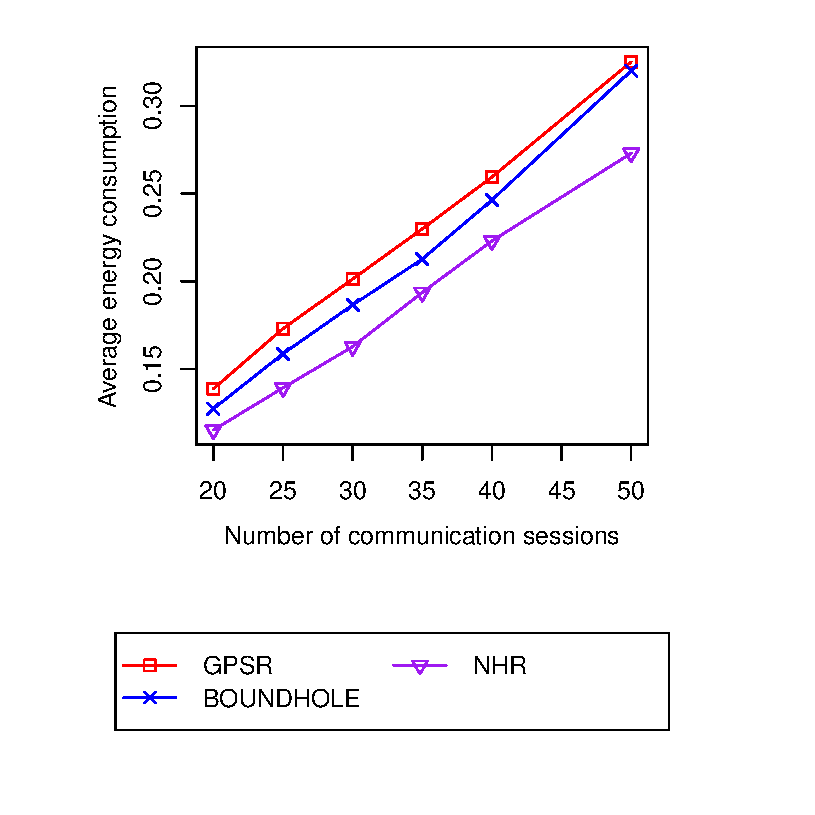
\includegraphics[width=0.6\textwidth]{Chapter7/Chapter7Figs/energy.eps}
\caption{Comparison of average energy consumption}
\label{fig-energy}
\end{figure}


\section{Deviation of energy consumption}
The deviation of energy consumption is calculated by the following formula: $\sigma = \sqrt{\frac{1}{K}\sum_{i=1}^{K}\left ( e_i - \frac{\sum_{i=1}^{K}e_i}{K} \right )^2}$, where $K$ is number of sensor nodes and $e_i$ is energy consumed by the $i^{th}$ node. The deviation of energy consumption of sensor nodes can give us a view of energy balancing. The more even the distribution of energy consumption is the better load balancing the protocol achieves. The smaller the deviation is, the higher the load balancing of network will be. 

\begin{figure}[!htb]
  \centering
  \captionsetup{justification=centering}
  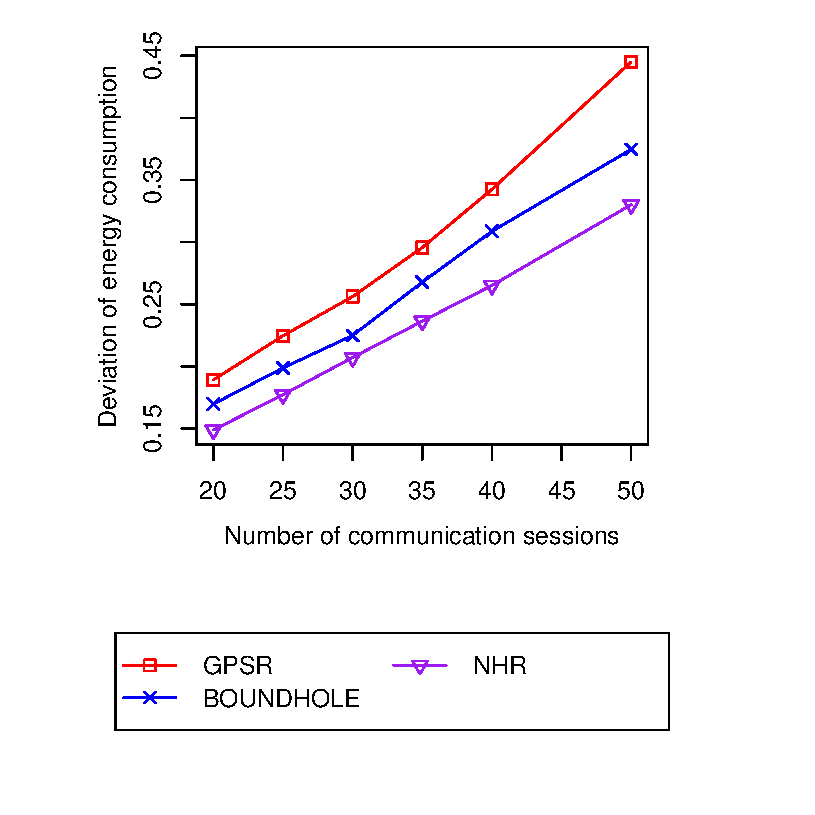
\includegraphics[width=0.6\textwidth]{Chapter7/Chapter7Figs/dev.eps}
\caption{Comparison of deviation of energy consumption}
\end{figure}

\section{Energy consumption of individual sensor nodes}
Figure \ref{fig-3d} scatters the energy consumption of individual sensor nodes in 3-dimension graphs. These figures give us a visual view of load balancing status of network. It is clear that, the per-node energy consumption by using GPSR and BOUNDHOLE are the most imbalanced. This imbalance is illustrated best by a look at the peaks at the center of figure \ref{fig-3d-gpsr}, \ref{fig-3d-boundhole}. The position of the peaks correspond to the location of the hole.
\begin{figure}[!htb]
\centering
\begin{subfigure}{0.5\textwidth}
  \centering
  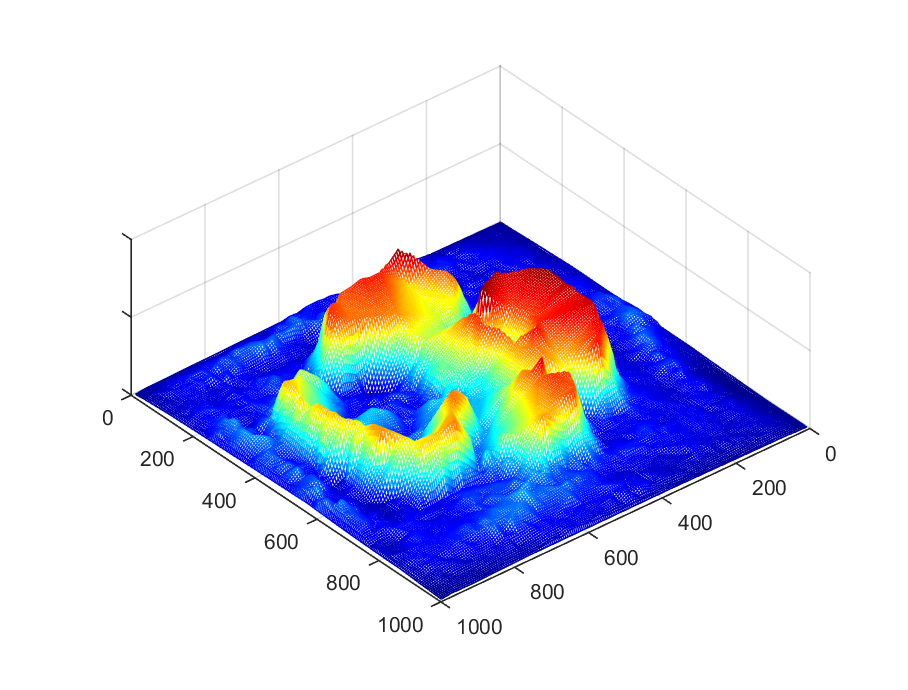
\includegraphics[width=0.8\textwidth]{Chapter7/Chapter7Figs/gpsr-energy.eps}
  \caption{GPSR}
  \label{fig-3d-gpsr}
\end{subfigure}%
\begin{subfigure}{0.5\textwidth}
  \centering
  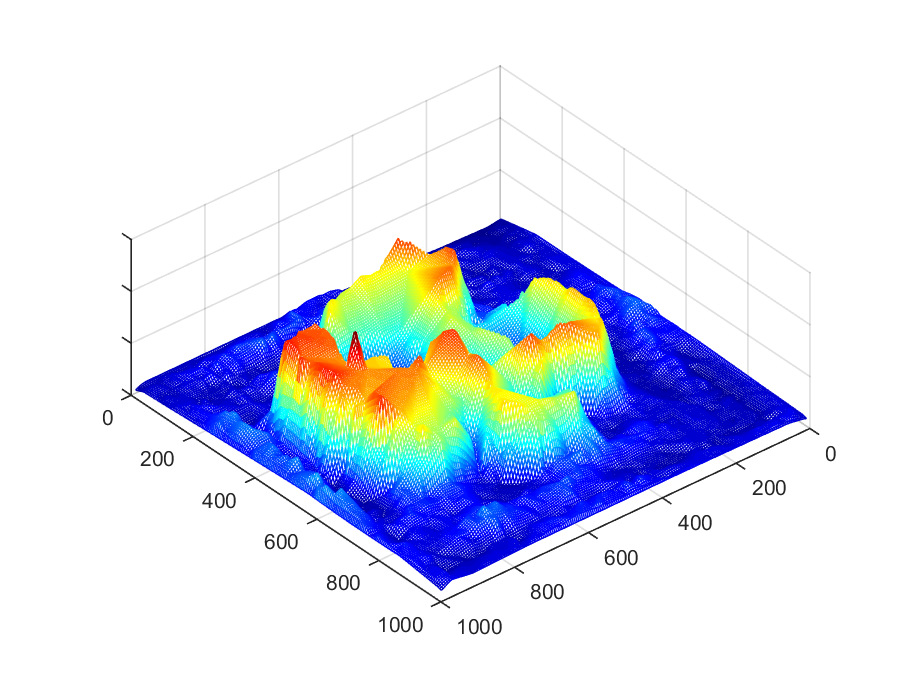
\includegraphics[width=0.8\textwidth]{Chapter7/Chapter7Figs/boundhole-energy.eps}
  \caption{BOUNDHOLE}
    \label{fig-3d-boundhole}
\end{subfigure}
\begin{subfigure}{0.5\textwidth}
  \centering
  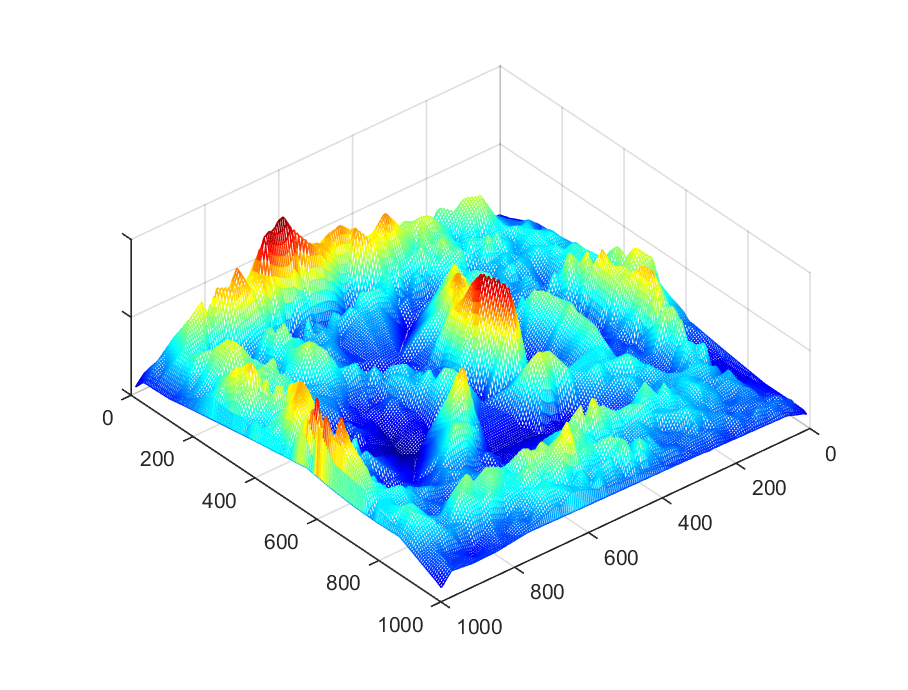
\includegraphics[width=0.8\textwidth]{Chapter7/Chapter7Figs/nhr-energy.eps}
  \caption{NHR}
\end{subfigure}
\caption{Visual view of energy consumption of individual sensor nodes}
\label{fig-3d}
\end{figure}

\section{Average path length}
The average path length is calculated as the average hop-count of all successfully transmitted packets. The comparison of the average path length for three protocols is shown in figure \ref{fig-path-length}.

\begin{figure}[!htb]
  \centering
  \captionsetup{justification=centering}
  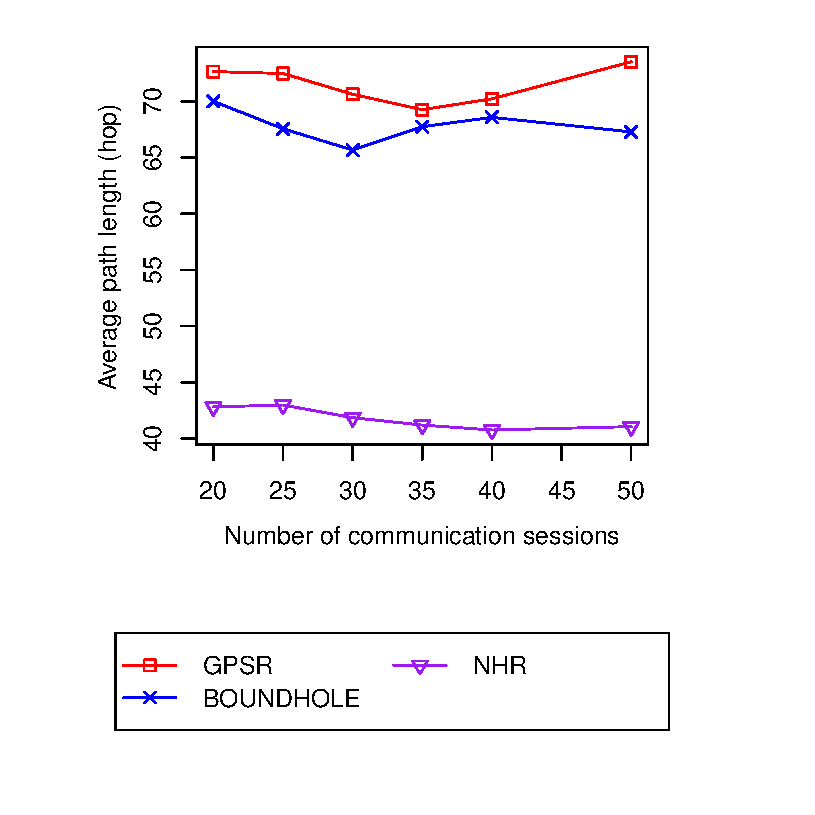
\includegraphics[width=0.6\textwidth]{Chapter7/Chapter7Figs/path.eps}
\caption{Comparison of average path length}
\label{fig-path-length}
\end{figure}

\section{Routing path stretch}
In this section we also evaluate the stretch by hop-count (i.e. the most practical stretch metric). The stretch by hop-count is the ratio between the hop-count of the routing path using routing protocol and the optimal path.

\section{Impact of $\delta$ on protocol}
We also conduct another experiment to investigate the impact of $\delta$ on the protocol. Three metrics are compared: the average path length, the average energy consumed, the deviation of energy consumption.

\begin{figure}[!htb]
\centering
\begin{subfigure}{0.5\textwidth}
  \centering
  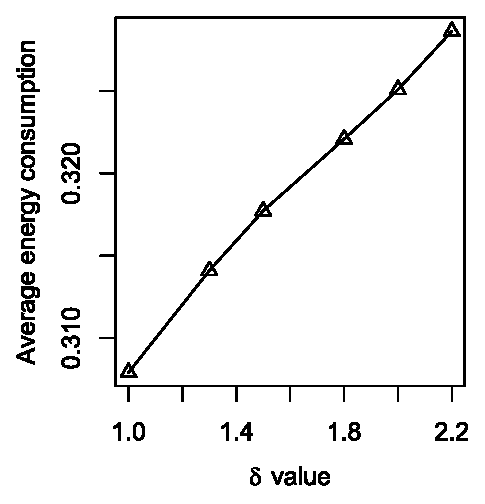
\includegraphics[width=0.8\textwidth]{Chapter7/Chapter7Figs/nhr-energy-plot.eps}
  \caption{Average energy consumption}
\end{subfigure}%
\begin{subfigure}{0.5\textwidth}
  \centering
  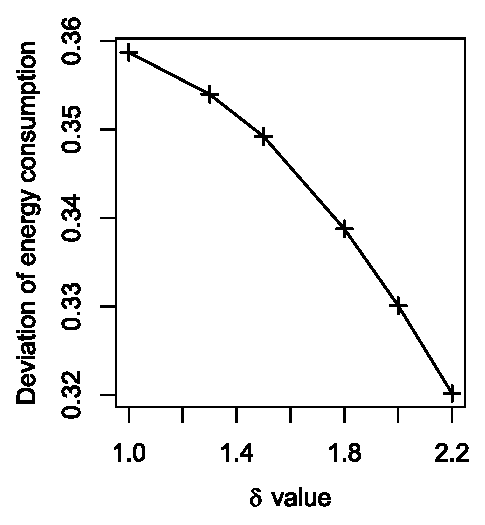
\includegraphics[width=0.8\textwidth]{Chapter7/Chapter7Figs/nhr-dev-plot.eps}
  \caption{Deviation of energy consumption}
\end{subfigure}
\begin{subfigure}{0.5\textwidth}
  \centering
  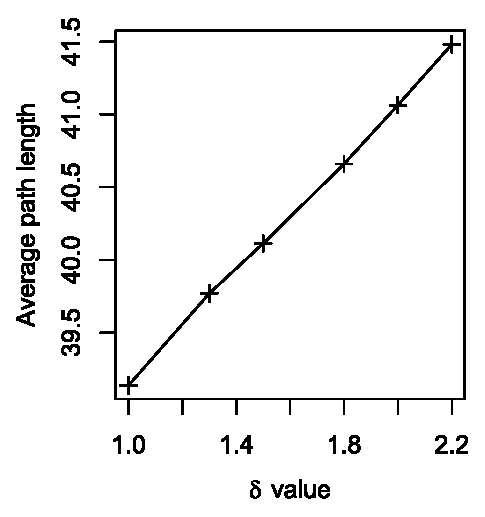
\includegraphics[width=0.8\textwidth]{Chapter7/Chapter7Figs/nhr-path-plot.eps}
  \caption{Average path length}
\end{subfigure}
\caption{Impact of $\delta$ on: average energy consumption, deviation of energy consumption and average path length}
\end{figure}
